\section{Controller}

  This chapter describes the implementation of the features elicited on the previous chapters in details, specifically within the FDS component. All the HTTP routes of the FDS will be prefixed with \verb;/api/v1;.

  \subsection{Customer Validation on a Registration Event}

    An HTTP endpoint will be implemented to provide the possibility to schedule a validation process as soon as a new customer is registered. The endpoint should accept the customer information on the request body and return validation ID and additional information of the validation process as a response. 
    
    The HTTP controller is intentionally kept as simple as possible. The logic behind the process to schedule a validation is done by the \verb;ValidationService; and \verb;ValidationEngine; (discussed in \autoref{sub:process}). The \verb;ValidationService; is responsible in this particular case to get the lists of existing validation rules and runtime secrets, then creating a new instance of \verb;ValidationEngine; as well as scheduling a new validation process. 

  \subsection{Validation Process}
    \label{sub:process}

    \subsubsection{Validation Process Flow}
    
      A validation process is started by iterating through a list of validation rules, making an HTTP request to the external endpoint listed on each rule and evaluating its response in comparison to the conditions attached on the rule. If the HTTP response from the external matches the conditions of the rule, the rule evaluation will be considered as a passed evaluation, otherwise it is a failed evaluation. The result of each rule evaluation determines the value of the resulting fraud score. The resulting fraud score will be calculated as follows: 

      \begin{itemize}
        \item Initialize an empty list of fraud scores. The list will be filled later with float numbers ranging between 0 and 1
        \item Go through the list of validation rules and run evaluation
        \item If the evaluation passed, append \verb;0; to the list of fraud scores
        \item Otherwise, append the validation rule \verb;failScore; attribute's value to the list of fraud scores
        \item At the end of the iteration, the list size should equal to the amount of available\footnote{\emph{Not skipped.}} validation rules
        \item The resulting fraud score is the sum of the scores in the list, divided by the number of available validation rules
      \end{itemize}

      \begin{figure}[!ht]
        \centering
        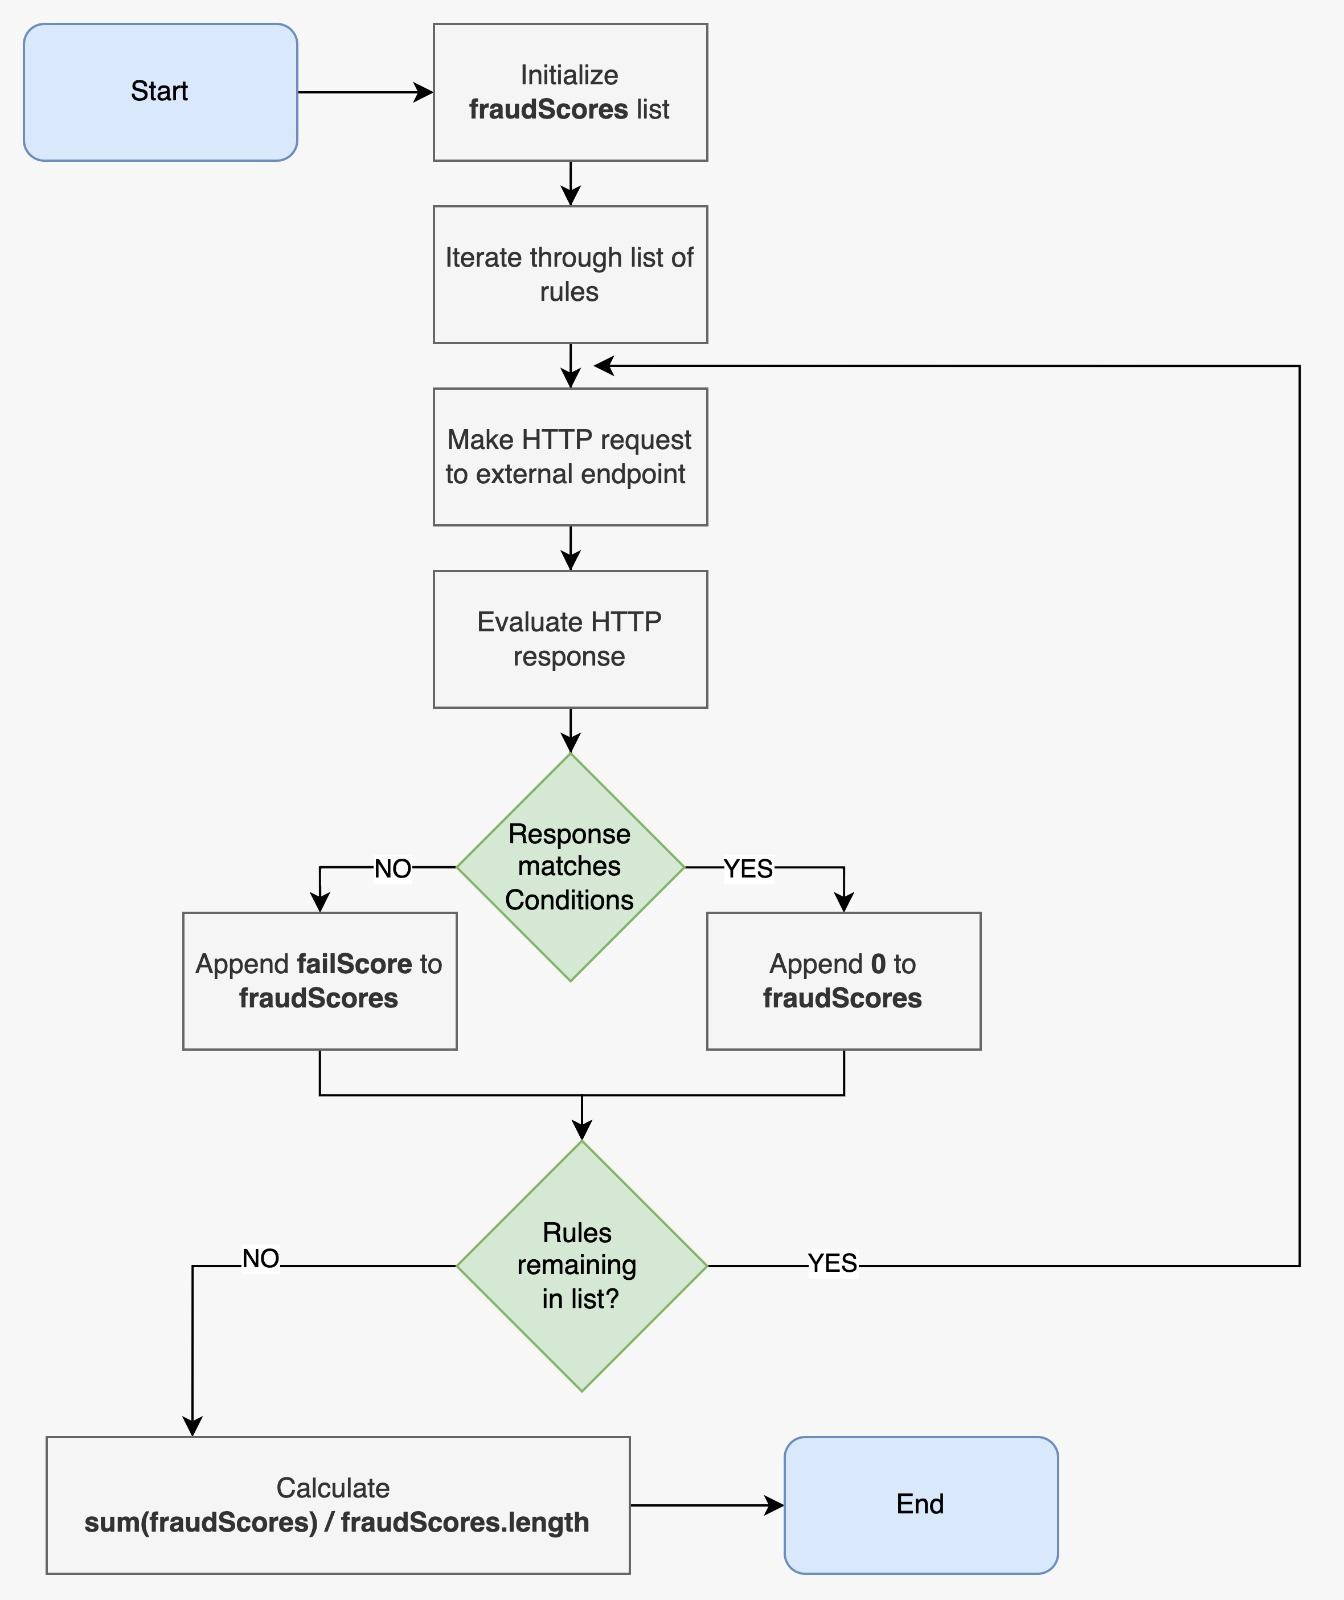
\includegraphics[width=0.8\textwidth]{diagrams/flow_validation_process.jpeg}
        \caption{Flow diagram of a validation process}
        \label{fig:flow_validation}
      \end{figure}
      
      The flow listed above will be executed by creating a \verb;ValidationEngine; instance and calling a public \verb;secheduleRulesetValidation; method. Before running a validation process, the list of validation rules as well as runtime secrets\footnote{Runtime secrets are used to store confidential information such as API keys.} should be provided to the engine. The \verb;ValidationEngine; class uses method chaining\footnote{\emph{Method chaining} is a way to provide the possibility of invoking multiple method calls of an object without having to store an intermediary result in an additional variable.} as well as the \emph{Builder} design pattern discussed in \autocite[pp. 97-106]{gamma-1995} for its construction, to make the public API of a validation engine as simple as possible.

      \begin{lstlisting}[style=es6, caption={ValidationEngine class builder pattern using method chaining (TypeScript)}]
export class ValidationEngine<T> {
  private secrets: GenericObject = {}
  private ruleset: ValidationRule[] = []

  setSecrets(secrets: GenericObject) {
    this.secrets = secrets
    return this
  }

  setRuleset(ruleset: ValidationRule[]) {
    this.ruleset = [...ruleset.sort((a, b) => b.priority - a.priority)]
    return this
  }
}
      \end{lstlisting}

    \subsubsection{Accessing Data by Evaluating JSONPath Expressions}
      
      To be able to access essential information stored in the current runtime scope a validation process, a JSONPath expression can be used in certain attributes of a validation rule. The provided runtime information of a validation process includes the customer information, runtime secrets and during a condition evaluation, the HTTP response from the external endpoint of the particular rule. 

      The ability to access certain information from the runtime scope is needed when an HTTP request is made and during the evaluation of a condition. To evaluate a JSONPath expression, the \verb;jsonpath; library is used. 

      \begin{lstlisting}[style=es6, caption={Accessing runtime information using JSONPath expression (TypeScript)}]
import jp from "jsonpath"

const accessDataFromPath = (runtimeData: any, expression: any) => {
  if (typeof expression !== "string") {
    return expression // A valid JSONPath expression is a string
  }
  
  try {
    const [dataFromPath] = jp.query(runtimeData, expression)
    if (!dataFromPath) {
      // Expression is valid, but the path doesn't point to a specific value
      return expression 
    }

    return dataFromPath
  } catch {
    return expression // The expression is either not a valid JSONPath expression
  }
}
      \end{lstlisting}

    \subsubsection{Making an HTTP Request to External Endpoints}

      A dedicated class (\verb;Agent;) is created to make an HTTP request to the external endpoint. The class will provide a layer of abstraction on top of the Got library that is being used to actually make the HTTP requests. 
      
      The class will also help in setting the request body, request header as well as to change the variables on the \verb;endpoint; attribute with its corresponding values. The class follows the \emph{Singleton} design pattern described in \autocite[pp. 127-134]{gamma-1995}, as there might only one instance needed for the whole application. The class is also implemented using the dependency injection in mind, for an easier access to the underlying library during the testing phase. The dependency injection is implemented by providing a \verb;context; object to the \verb;Agent; class beforehand. During runtime, the \verb;context; object contains a Got instance, used to make HTTP requests. In testing environment, the \verb;context; object contains a mocked Got instance.

      \begin{lstlisting}[style=es6, caption={Usage of the singleton pattern and dependency injection in Agent class (TypeScript)}]
export class Agent {
  private static context: Context // Dependency injection

  private static get client() {
    return Agent.context.client // `client` object is a Got instance
  }

  static setClient(context: Context) {
    this.context = context
  }
}
      \end{lstlisting}

    \subsubsection{Operators}

      \verb;Operators; are special classes that define the operation of a certain condition during a validation process. Each \verb;Operator; is grouped by its type and has two main properties \verb;identifier;, and \verb;operateFunction;
      
      The \verb;identifier; property of an operator refers to the operator's name, unique on its group of type. The \verb;identifier; attribute of an operator will be passed into the \verb;operator; attribute of a condition to describe the specific operator to be used in evaluating the particular condition. The \verb;operateFunction; attribute of an operator is a function that accepts two arguments, and returns a boolean value that indicates whether the operation is successful. An additional validation process is also implemented using the \verb;validateFunction; property to make sure that the value being passed into the \verb;operate; function of an operator is valid. The \verb;identifier; and \verb;operateFunction; attributes of an operator are passed into the object constructor during its initialization, while the \verb;validateFunction; attribute of an operator is defined by each subclass of the operator, grouped by its type.  
      
      \begin{lstlisting}[style=es6, caption={NumberOperator example (TypeScript)}]
export class NumberOperator extends Operator<number, NumberOperatorIds> {
  const validateFunction = (value) =>
    typeof value === "number" &&
    !isNaN(parseFloat(`${value}`))
}

export const numberOperators: Record<NumberOperatorIds, NumberOperator> = {
  eq: new NumberOperator("eq", (a, b) => b === a),
  gt: new NumberOperator("gt", (a, b) => b > a),
  gte: new NumberOperator("gte", (a, b) => b >= a),
  lt: new NumberOperator("lt", (a, b) => b < a),
  lte: new NumberOperator("lte", (a, b) => b <= a),
} 
      \end{lstlisting}

      The \emph{Flyweight} design pattern mentioned in \autocite[pp. 195-206]{gamma-1995} is used here, by instantiating all the available operators beforehand, and using the instantiated object during a condition evaluation. For an even easier access to the operators, a \emph{flyweight factory} is also created. The \verb;OperatorFactory; will return the appropriate operator to be used based on the type and identifier passed. If the combination of type and identifier of an operator doesn't point into a specific operator, a \verb;NullishOperator; will be returned, which always return \verb;false; as its operation result. 

    \subsubsection{Evaluating a Rule} 
      
      To evaluate a certain validation rule, the \verb;Evaluator; class is created. The \verb;Evaluator; class is responsible in running an evaluation regarding a certain condition. An evaluator works together with the \verb;Operator; class in evaluating the conditions given. The specific operator to evaluate a condition is accessed via the \verb;OperatorFactory;. The \verb;Evaluator; class encapsulates the internal logic of evaluating a condition and running the operations defined by the particular condition. The \verb;Evaluator; class is also responsible in accessing the required data described by a JSONPath expression from the runtime information of a validation process. 

      \begin{lstlisting}[style=es6, caption={The usage of OperatorFactory class in the Evaluator class (TypeScript)}]
// Evaluate JSONPath expressions.
const dataFromPath = this.accessDataFromPath(runtimeData, validationRule.path)
const valueFromPath = this.accessDataFromPath(runtimeData, validationRule.value)
        
const operator = OperatorFactory.getOperator(
  validationRule.type,
  validationRule.operator,
)
const isEvaluationPassed = operator.operate(valueFromPath, dataFromPath)
      \end{lstlisting}
      
      As mentioned before, a condition can either be a single condition, or multiple conditions, wrapped inside an \verb;any; or \verb;all; attribute. The evaluation of a single condition is different from the evaluation of multiple conditions. To facilitate the different logic of evaluating conditions, two subclasses of the \verb;Evaluator; class is created. \verb;ConditionEvaluator; is responsible in evaluating a single condition, while the \verb;BooleanConditionEvaluator; is in charge in evaluating multiple conditions and handling the logic behind evaluating the \verb;any; and \verb;all; modifier. To simplify the instantiation of the suitable \verb;Evaluator; subclass, the \verb;EvaluatorFactory; class is created, following the \emph{Factory Method} design pattern described in \autocite[pp. 107-116]{gamma-1995}. 

      \begin{lstlisting}[style=es6, caption={EvaluatorFactory usage in ValidationEngine class (TypeScript)}]
const response = await Agent.fireRequest(rule, {
  customer: customerData,
  secrets: this.secrets
})

const evaluator = EvaluatorFactory.getEvaluator(condition)
const evaluationResult = evaluator.evaluate({
  response: response.data,
  customer: customerData,
  secrets: this.secrets
})
      \end{lstlisting}

      As the evaluation result, an \verb;Evaluator; instance will return an object with the \verb;pass; attribute to determine whether the evaluation passed and an additional \verb;messages; attribute, which contains essential information regarding the evaluation (including the value of \verb;failMessage; attribute of a condition, if the evaluation fails). 

  \subsection{Notification on Suspicious Cases}
      
    In \autocite{amqp}, Subramoni et al. describes an exchange as a routing mediator that copies and send the message sent by a message publisher to zero or more message queues. The FDS acts as the message publisher of the system and publishes a message to a pre-defined exchange on every completion of a validation process. 
    An interface to access and publish a message to the exchange is implemented using the \emph{Singleton} \autocite[pp. 127-134]{gamma-1995} design pattern, to only have a single connection to the RabbitMQ, since an AMQP connection are designed to be long-lived and opening a new connection to a RabbitMQ instance is an expensive operation. The type of exchange used in the system is the \emph{fanout} exchange. When a message is published to a fanout exchange, the message will be routed to all the queues bound to the exchange, which is ideal for the use case of the current notification system. 

    \begin{lstlisting}[style=es6, caption={Openning a connection to RabbitMQ instance (TypeScript)}]
import { Channel, connect } from "amqplib"
export class Notification {
  private static channel: Channel | null = null

  async init(url: string) {
    try {
      const connection = await connect(url)
      const channel = await connection.createChannel() // Create a new channel
      // Assert whether the exchange exists, create new if it doesn't exist
      await channel.assertExchange("FDS", "fanout", {
        durable: true 
      }) 

      Notification.channel = channel
    } catch (err) {
      console.error(err)
    }
  }
}
    \end{lstlisting}
    
    The \verb;Notification; class also provides the \verb;publish; static method, which can be used to publish a new message to the exchange if the connection is opened successfully. The \verb;ValidationEngine; class calls the \verb;publish; method every time a validation process is completed, publishing the validation result of the particular validation process to the exchange.

    \begin{lstlisting}[style=es6, caption={Publishing a validation result to the RabbitMQ exchange (TypeScript)}]
Notification.publish(JSON.stringify(this.validationResult))
    \end{lstlisting}
    
    There can be many consumers consuming the messages published to the exchange, and run certain actions regarding the internal logic of the system itself. The message consumer can, for example email the concerned parties if the fraud score exceeds a certain threshold or even automatically block a customer if a specific rule evaluation failed. To consume a message published to the exchange, a connection to the RabbitMQ instance needs to be opened, and a dedicated message queue (ideally created only for internal usage of the consumer itself) is needed. 

    \newpage
    \begin{lstlisting}[style=es6, caption={Consuming a message published to the RabbitMQ exchange (TypeScript)}]
import { connect } from "amqplib"
export const start = async (url: string) => {
  try {
    const connection = await connect(url)
    const channel = await connection.createChannel()
    await channel.assertExchange("FDS", "fanout", { durable: true })
    // Create an exclusive queue (created only for internal usage)
    const { queue } = await channel.assertQueue("", { exclusive: true })

    // Bind the exclusive queue to the exchange
    channel.bindQueue(queue, "FDS", "") 

    await channel.consume(queue, async (message: string) => {
      // Do actions
    }, {
      noAck: true
    })
  } catch (err) {
    console.error(err)
  }
}
    \end{lstlisting}

  \subsection{Database Connection}
  
    To manage the validation rules and runtime secrets, a database connection to modify the database entries via the ORM (Prisma) is required. The \emph{Singleton} \autocite[pp. 127-134]{gamma-1995} design pattern is also used here to make sure, that only a single connection to the database is created. \emph{Dependency injection} is also used here to be able to provide a mocked Prisma instance during testing. 

    Caching can also be enabled in the \verb;Database; class, by providing a \verb;DataStore; instance to the static \verb;setCache; method. By enabling caching, the values retrieved and updated can be cached to provide a faster response time\footnote{Runtime secrets are not cached.}. 

  \subsection{Validation Real Time Progress}
    \label{impl_sse}
  
    The \emph{Observer} \autocite[pp. 293-303]{gamma-1995} will also be implemented here to provide the functionality of a real time progress update of a certain validation process. An \verb;EventEmitter; is used here to subscribe and publish certain events during a validation process. The FDS publishes a \verb;validation_event:update; event whenever a rule evaluation is done, containing the validation ID on the name of the event and sending the current validation result on the payload. When the particular validation process is done, the FDS also publishes a \verb;validation_done; event, containing the validation ID on the name of the event, as an indicator that the validation process is completed and no further events with the attached validation ID will be sent. 

    \begin{lstlisting}[style=es6, caption={Publishing events to the EventEmitter on certain validation events (TypeScript)}]
// Published when a rule evaluation is completed
EventBus.emit(
  `${EventBus.EVENTS.VALIDATION_EVENT_UPDATE}--${validationId}`,
  this.validationResult,
)
// Published when a validation process is completed
EventBus.emit(`${EventBus.EVENTS.VALIDATION_DONE}--${this.validation.validationId}`)
    \end{lstlisting}
    
    To continually provide a client with the latest progress of a validation event without having to provide a dedicated instance of a WebSocket server, the Server-Sent Events (SSE)\autocite{rfc8895} technology is used. The SSE enables the possibility to send new data to the client multiple times by only opening a single HTTP connection. 
    
    The difference between SSE and the WebSocket protocol, is that SSE only enables a one-way communication from server to client, meaning the client cannot continually send any new messages to the server. SSE is enough for the use case of the project, as the client doesn't need to send new data to the client to display real time progress of a validation process.

    The SSE is implemented by setting the \verb;Content-Type; header of the HTTP response to \verb;text/event-stream; and setting the \verb;Connection; header to \verb;keep-alive;. The \verb;Connection: keep-alive; header is useful to keep the connection between client and server open, while the \verb;Content-Type: text/event-stream; header specifies the type of message sent to the client. A message written to the event stream is prefixed with a \verb;"data: "; prefix. 

    After the header of the response is set, the FDS will push a new message to the stream whenever there's a new event emitted on the \verb;EventEmitter; with the corresponding validation ID. 

    \begin{lstlisting}[style=es6, caption={Writing to SSE stream when certain events are published (TypeScript)}]
static async subscribeToValidationProgress (
  validationId: string,
  responseObject: Response,
) {
  const updateEvent = `${EventBus.EVENTS.VALIDATION_EVENT_UPDATE}--${validationId}`
  const closeEvent = `${EventBus.EVENTS.VALIDATION_DONE}--${validationId}`

  EventBus.once(closeEvent, () => {
    closeConnection()
  })

  EventBus.on(
    updateEvent,
    (validationResult: Validation) => {
      writeToStream(validationResult)
    },
  )

  const writeToStream = (data: any) =>
    responseObject.write(
      `data: ${JSON.stringify(data)}\n\n`,
    )
}
    \end{lstlisting}

